\documentclass{article}
\usepackage{graphicx}
\usepackage{hyperref}
\usepackage{float}
\usepackage{booktabs}
\usepackage{multirow}
\usepackage[margin=1in]{geometry}

\title{Assignment 4 - Decision Tree\\
       Analysis Report}
\author{Gourove Roy\\
        2105017\\
        Bangladesh University of Engineering and Technology (BUET)}
\date{\today}

\begin{document}
\maketitle

\section*{Introduction}
This report presents the results of decision tree experiments on the Iris and Adult datasets using three attribute selection criteria: Information Gain (IG), Information Gain Ratio (IGR), and Normalized Weighted Information Gain (NWIG). The experiments evaluated how different criteria and pruning depths affect accuracy, tree complexity, and overfitting behavior. The implementation followed the specifications in the assignment document, including handling of missing values and 20 repeated trials with random 80/20 splits.

\section*{Experimental Setup}
The decision tree was implemented in C++ with the following specifications:
\begin{itemize}
    \item \textbf{Datasets:} Iris (150 samples, 4 features) and Adult (48,842 samples, 14 features)
    \item \textbf{Attribute Selection:} IG, IGR, and NWIG criteria as defined in the assignment
    \item \textbf{Pruning:} Maximum depth parameter (0 = no pruning)
    \item \textbf{Missing Values:} Replaced with most common attribute value
    \item \textbf{Continuous Attributes:} Discretized into low/medium/high using 33rd/66th percentiles
    \item \textbf{Evaluation:} 20 trials with random 80\%/20\% splits, average accuracy reported
\end{itemize}

\section*{Results and Graphs}

\begin{figure}[H]
    \centering
    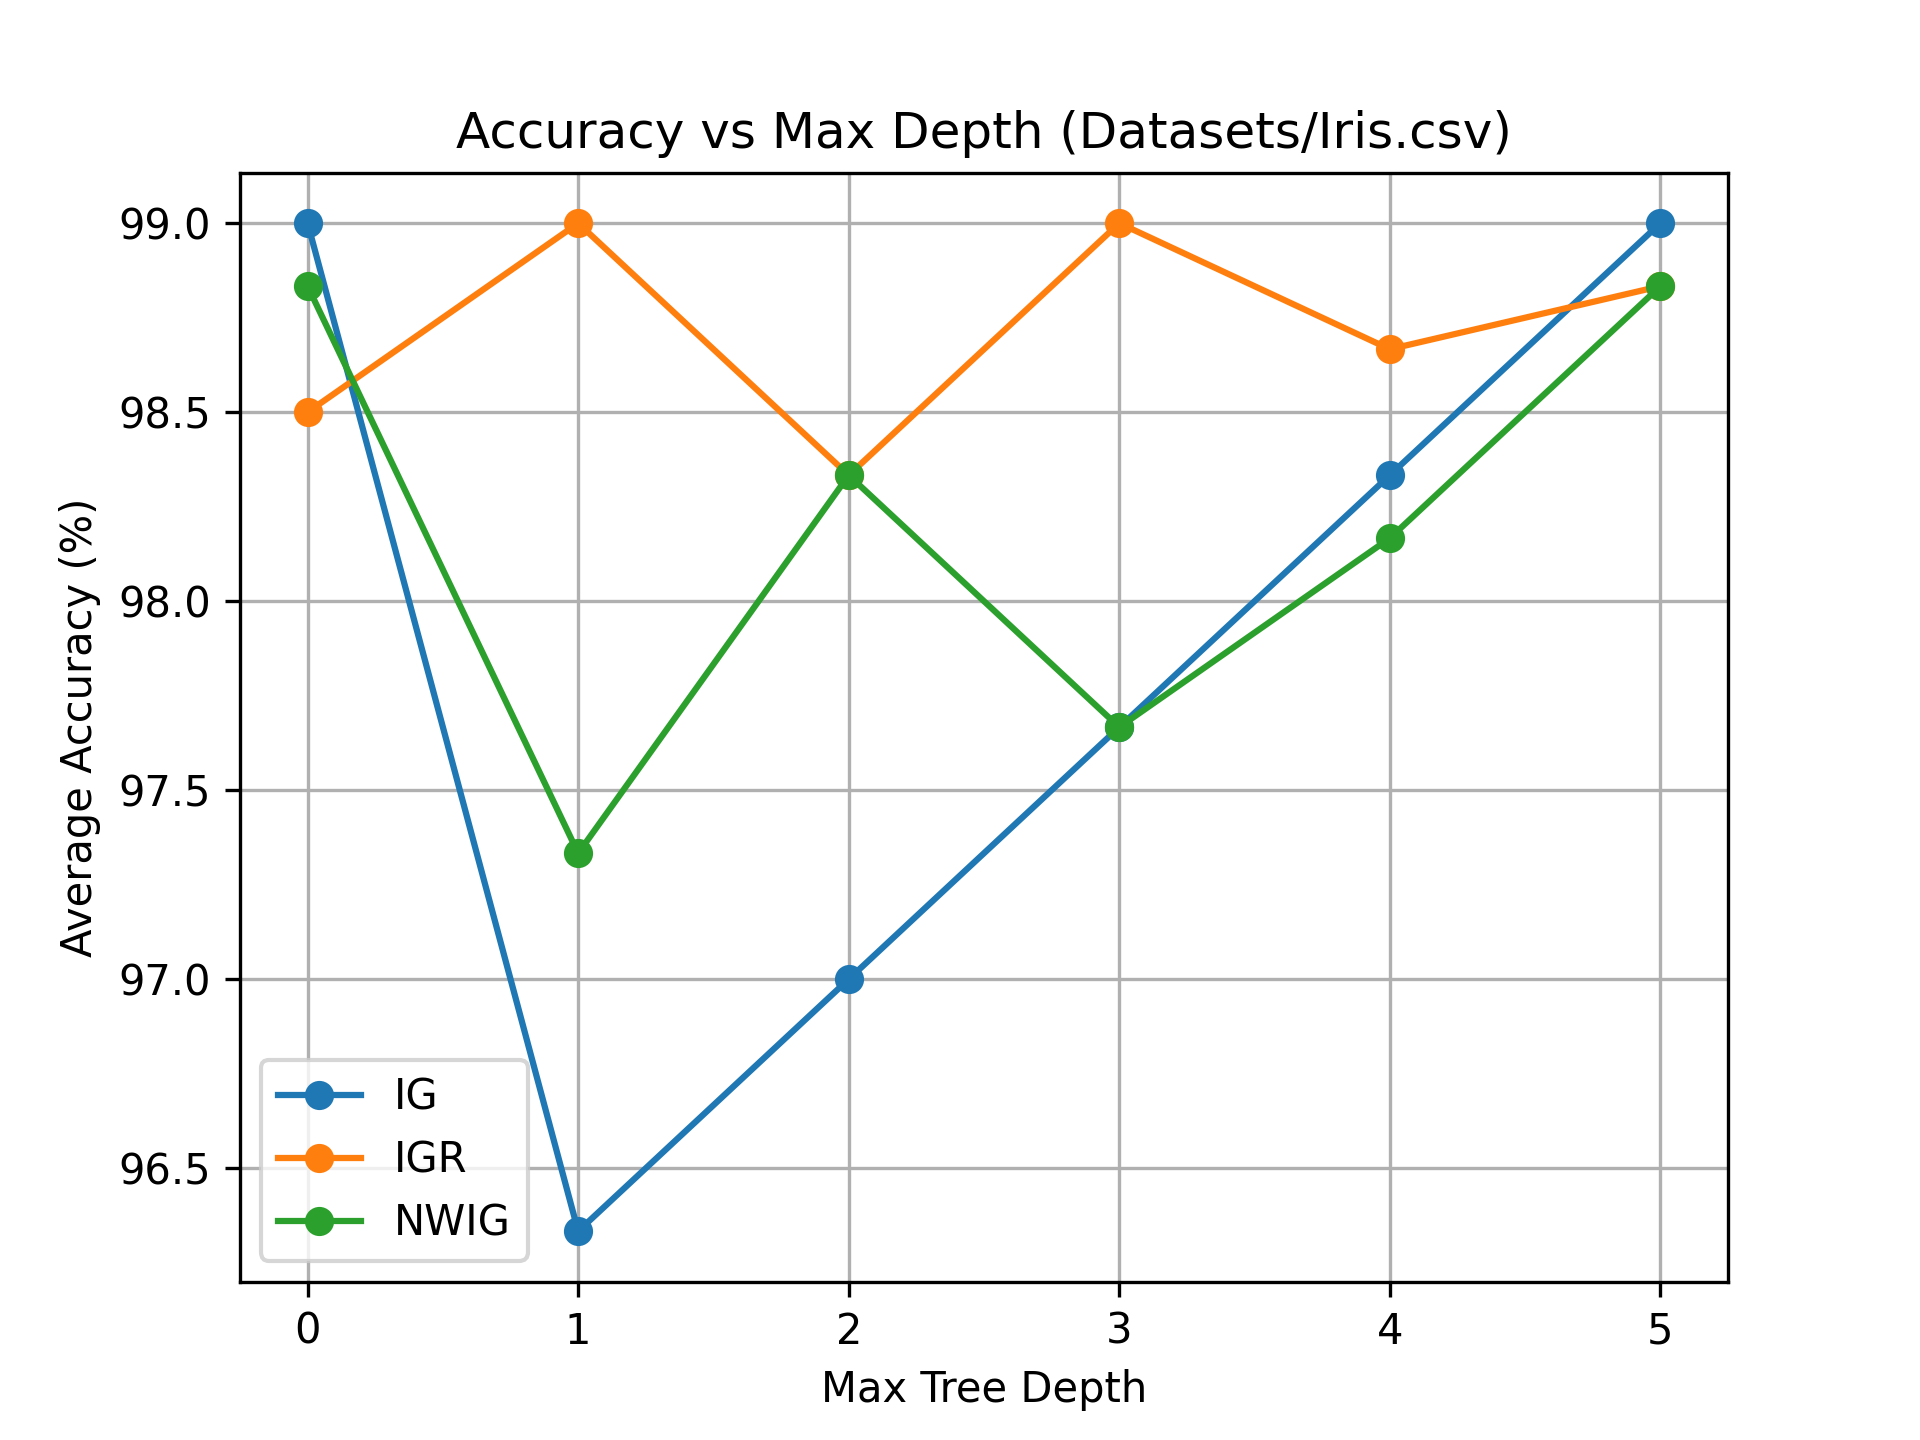
\includegraphics[width=0.75\textwidth]{analysis/images/Datasets_Iris.csv_accuracy.png}
    \caption{Average Accuracy vs Max Depth for Iris Dataset}
    \label{fig:iris_acc}
\end{figure}

\begin{figure}[H]
    \centering
    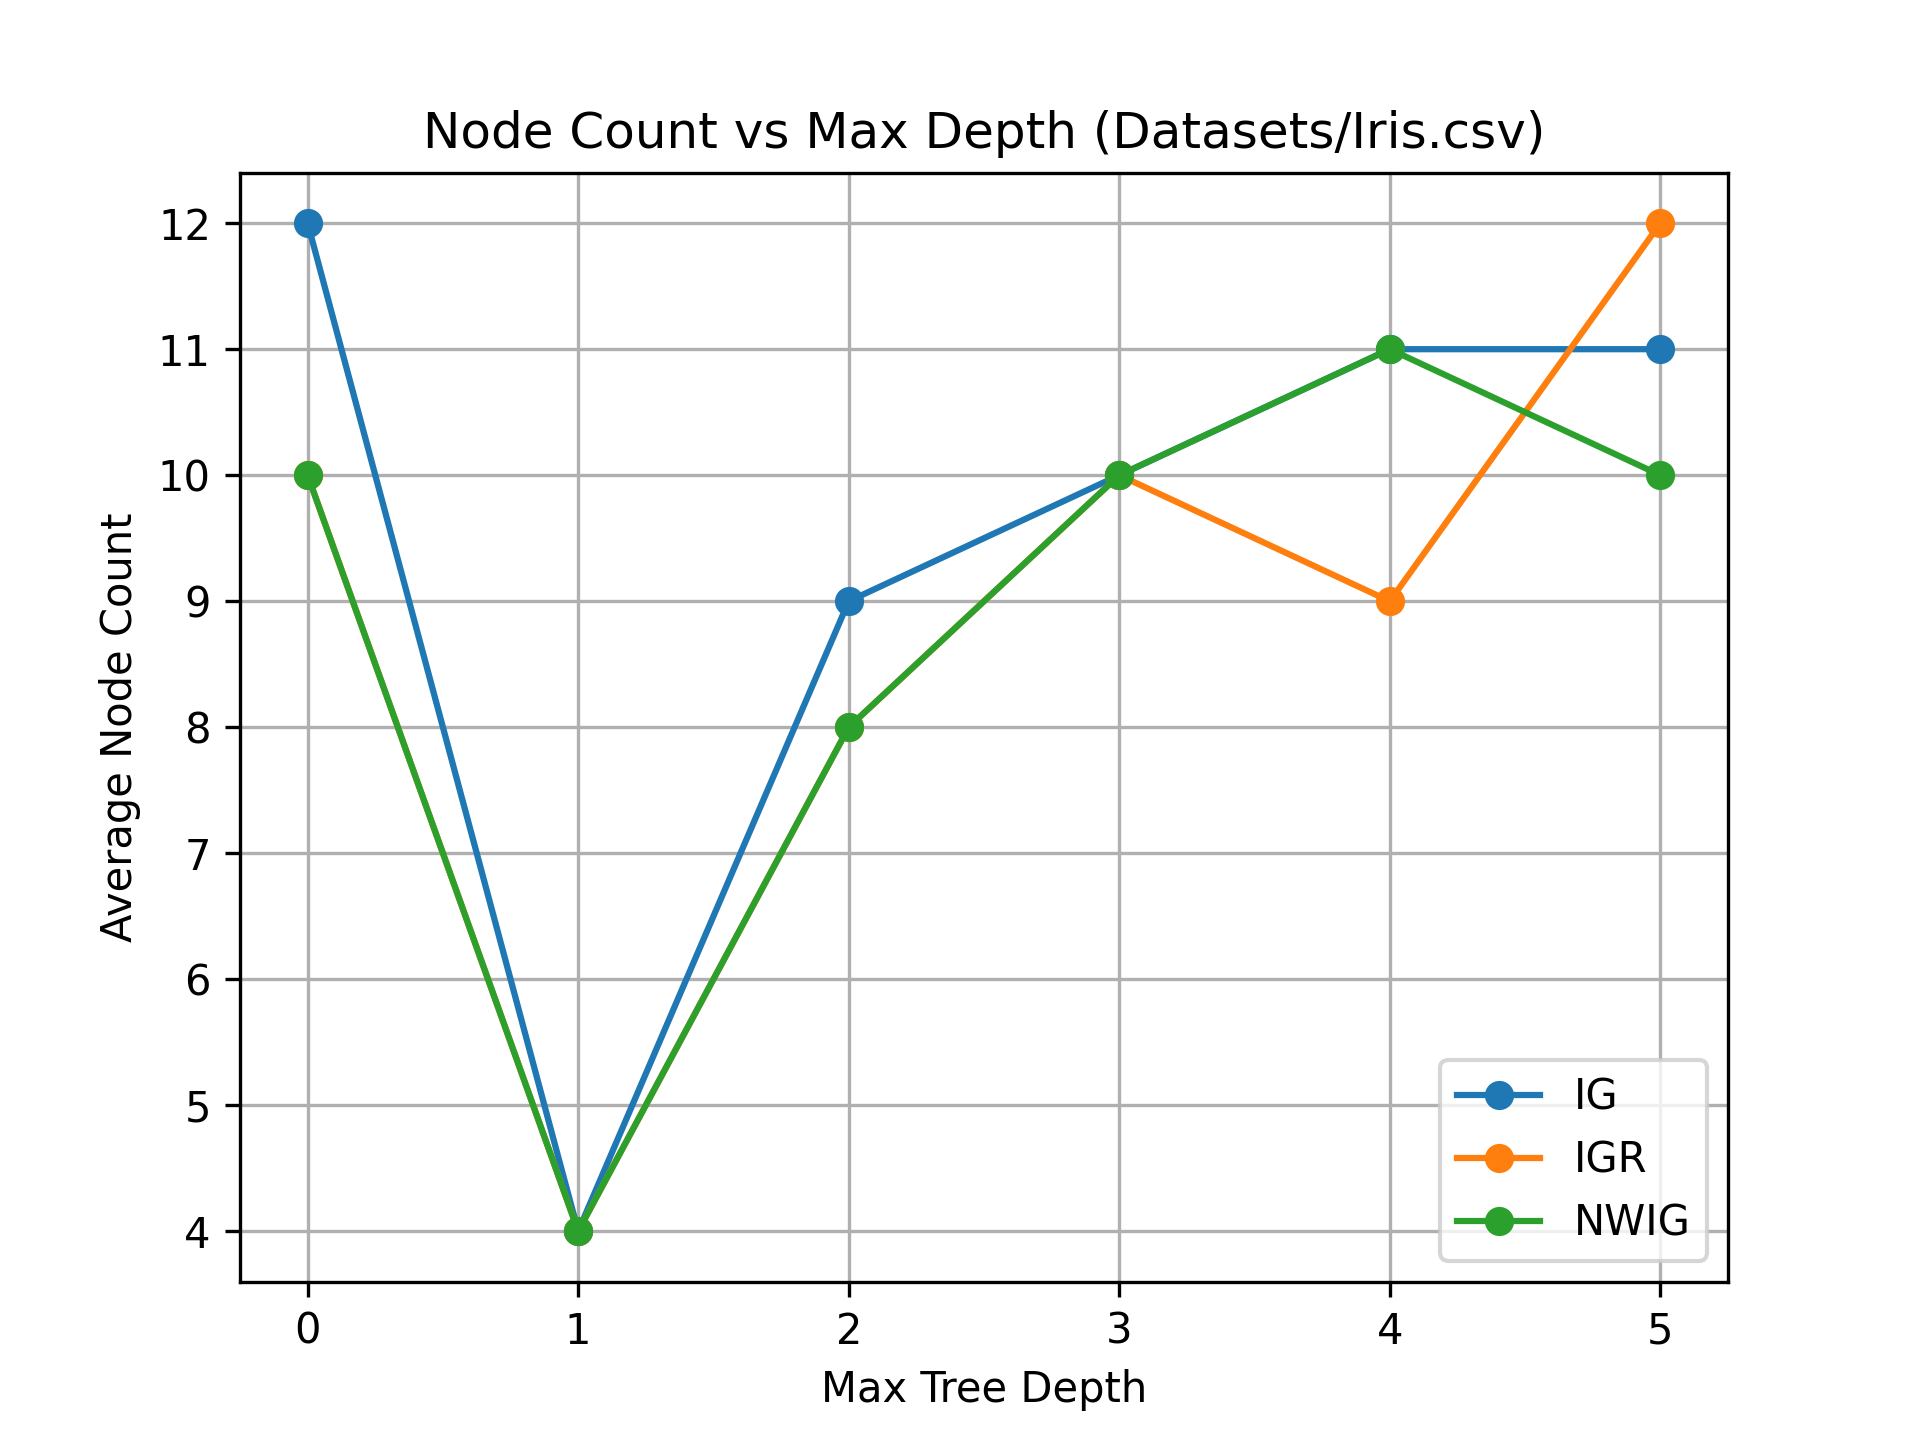
\includegraphics[width=0.75\textwidth]{analysis/images/Datasets_Iris.csv_nodes.png}
    \caption{Average Node Count vs Max Depth for Iris Dataset}
    \label{fig:iris_nodes}
\end{figure}

\begin{figure}[H]
    \centering
    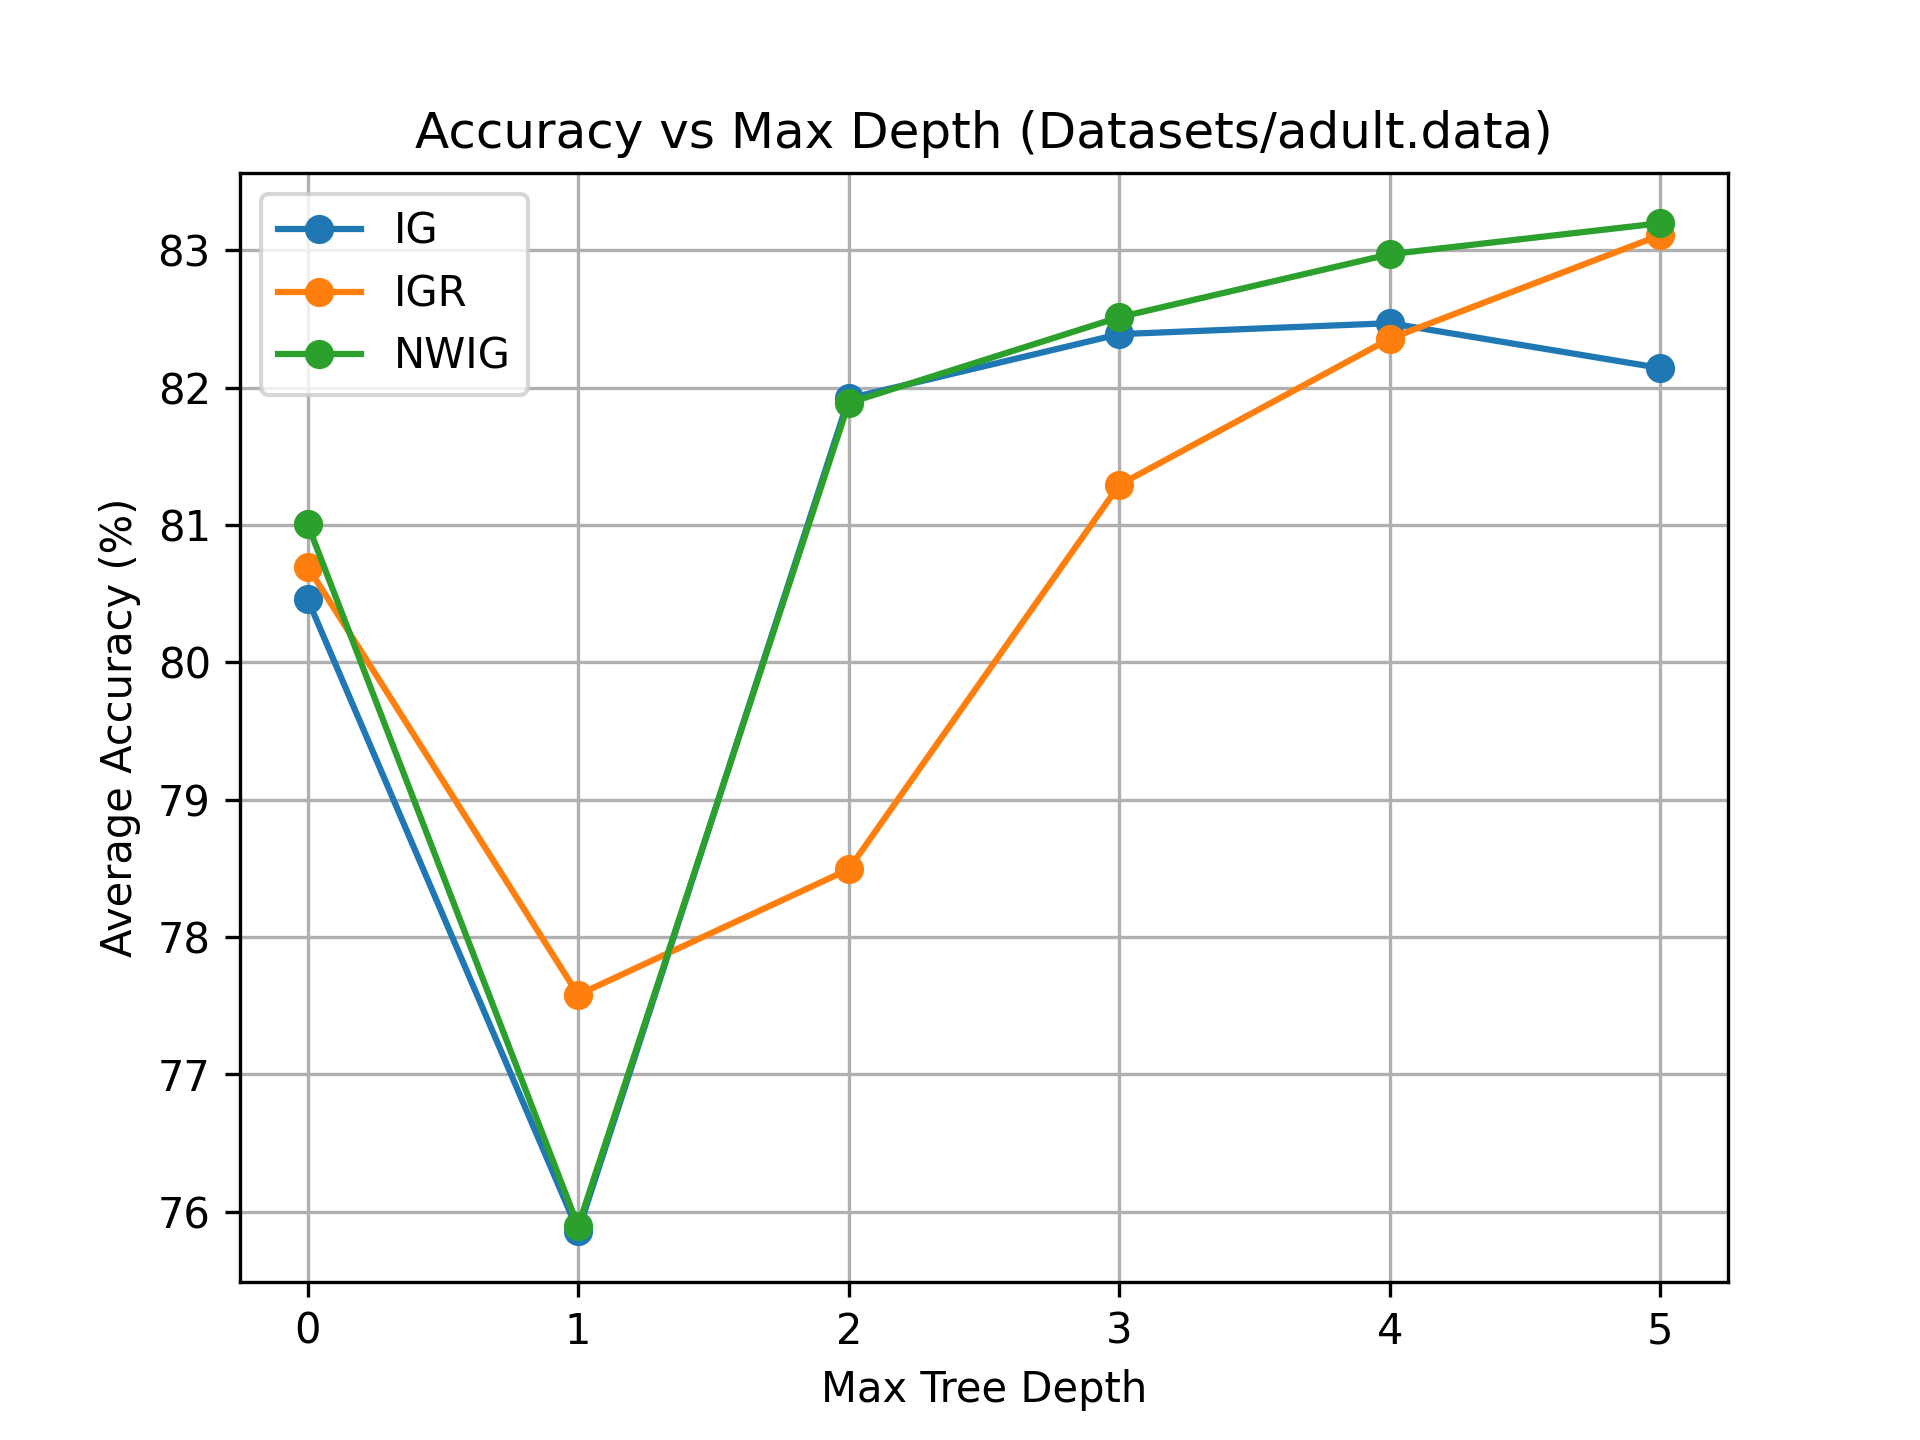
\includegraphics[width=0.75\textwidth]{analysis/images/Datasets_adult.data_accuracy.png}
    \caption{Average Accuracy vs Max Depth for Adult Dataset}
    \label{fig:adult_acc}
\end{figure}

\begin{figure}[H]
    \centering
    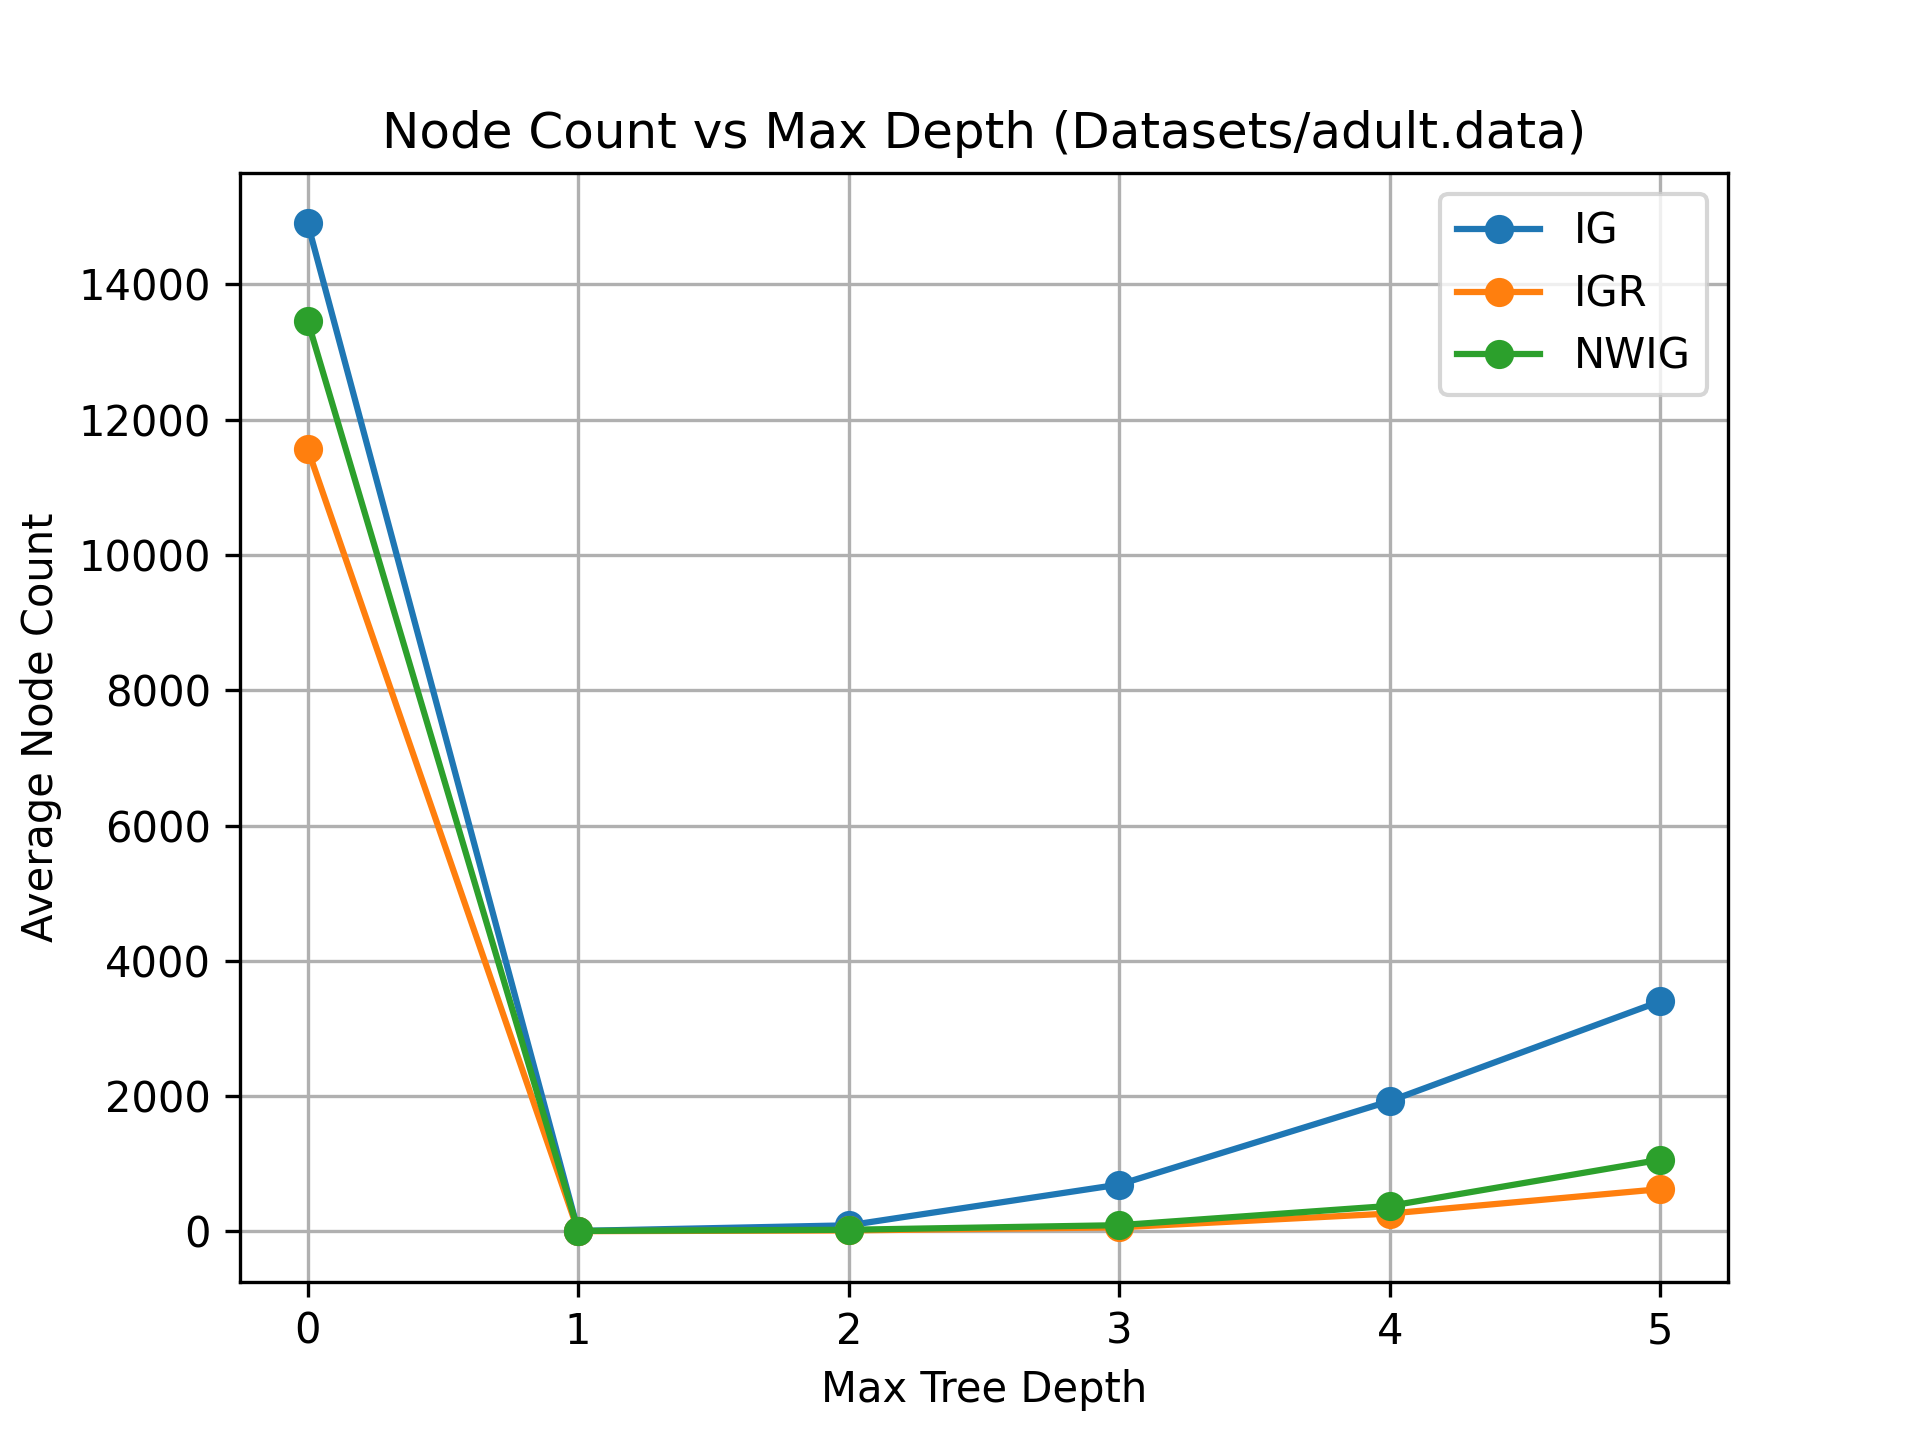
\includegraphics[width=0.75\textwidth]{analysis/images/Datasets_adult.data_nodes.png}
    \caption{Average Node Count vs Max Depth for Adult Dataset}
    \label{fig:adult_nodes}
\end{figure}

\section*{Detailed Results Tables}

\begin{table}[H]
\centering
\caption{Unpruned Tree Statistics (Max Depth = 0)}
\begin{tabular}{lccc}
\toprule
\multicolumn{1}{l}{\textbf{Dataset \newline Criterion}} & \textbf{Avg. Depth} & \textbf{Avg. Nodes} & \textbf{Avg. Accuracy} \\
\midrule
Iris (IG) & 4 & 12 & 0.99 \\
Iris (IGR) & 3 & 10 & 0.985 \\
Iris (NWIG) & 3 & 10 & 0.988 \\
\midrule
Adult (IG) & 14 & 14904 & 0.8046 \\
Adult (IGR) & 14 & 11569 & 0.8069 \\
Adult (NWIG) & 14 & 13463 & 0.8101 \\
\bottomrule
\end{tabular}
\label{tab:unpruned}
\end{table}

% Table 2: Max Depth = 1
\begin{table}[H]
\centering
\caption{Tree Statistics (Max Depth = 1)}
\begin{tabular}{lccc}
\toprule
\multicolumn{1}{l}{\textbf{Dataset \newline Criterion}} & \textbf{Avg. Depth} & \textbf{Avg. Nodes} & \textbf{Avg. Accuracy} \\
\midrule
Iris (IG) & 1 & 4 & 0.9633 \\
Iris (IGR) & 1 & 4 & 0.99 \\
Iris (NWIG) & 1 & 4 & 0.9733 \\
\midrule
Adult (IG) & 1 & 7 & 0.7586 \\
Adult (IGR) & 1 & 3 & 0.7758 \\
Adult (NWIG) & 1 & 7 & 0.7589 \\
\bottomrule
\end{tabular}
\label{tab:depth1}
\end{table}

% Table 3: Max Depth = 2
\begin{table}[H]
\centering
\caption{Tree Statistics (Max Depth = 2)}
\begin{tabular}{lccc}
\toprule
\multicolumn{1}{l}{\textbf{Dataset \newline Criterion}} & \textbf{Avg. Depth} & \textbf{Avg. Nodes} & \textbf{Avg. Accuracy} \\
\midrule
Iris (IG) & 2 & 9 & 0.97 \\
Iris (IGR) & 2 & 8 & 0.9833 \\
Iris (NWIG) & 2 & 8 & 0.9833 \\
\midrule
Adult (IG) & 2 & 90 & 0.8192 \\
Adult (IGR) & 2 & 14 & 0.7849 \\
Adult (NWIG) & 2 & 24 & 0.8189 \\
\bottomrule
\end{tabular}
\label{tab:depth2}
\end{table}

% Table 4: Max Depth = 3
\begin{table}[H]
\centering
\caption{Tree Statistics (Max Depth = 3)}
\begin{tabular}{lccc}
\toprule
\multicolumn{1}{l}{\textbf{Dataset \newline Criterion}} & \textbf{Avg. Depth} & \textbf{Avg. Nodes} & \textbf{Avg. Accuracy} \\
\midrule
Iris (IG) & 3 & 10 & 0.9767 \\
Iris (IGR) & 3 & 10 & 0.99 \\
Iris (NWIG) & 3 & 10 & 0.9767 \\
\midrule
Adult (IG) & 3 & 693 & 0.8239 \\
Adult (IGR) & 3 & 60 & 0.8129 \\
Adult (NWIG) & 3 & 92 & 0.8251 \\
\bottomrule
\end{tabular}
\label{tab:depth3}
\end{table}

% Table 5: Max Depth = 4
\begin{table}[H]
\centering
\caption{Tree Statistics (Max Depth = 4)}
\begin{tabular}{lccc}
\toprule
\multicolumn{1}{l}{\textbf{Dataset \newline Criterion}} & \textbf{Avg. Depth} & \textbf{Avg. Nodes} & \textbf{Avg. Accuracy} \\
\midrule
Iris (IG) & 3 & 11 & 0.9833 \\
Iris (IGR) & 3 & 9 & 0.9867 \\
Iris (NWIG) & 3 & 11 & 0.9817 \\
\midrule
Adult (IG) & 4 & 1927 & 0.8247 \\
Adult (IGR) & 4 & 264 & 0.8236 \\
Adult (NWIG) & 4 & 377 & 0.8297 \\
\bottomrule
\end{tabular}
\label{tab:depth4}
\end{table}

% Table 6: Max Depth = 5
\begin{table}[H]
\centering
\caption{Tree Statistics (Max Depth = 5)}
\begin{tabular}{lccc}
\toprule
\multicolumn{1}{l}{\textbf{Dataset \newline Criterion}} & \textbf{Avg. Depth} & \textbf{Avg. Nodes} & \textbf{Avg. Accuracy} \\
\midrule
Iris (IG) & 3 & 11 & 0.99 \\
Iris (IGR) & 4 & 12 & 0.9883 \\
Iris (NWIG) & 3 & 10 & 0.9883 \\
\midrule
Adult (IG) & 5 & 3402 & 0.8214 \\
Adult (IGR) & 5 & 625 & 0.8311 \\
Adult (NWIG) & 5 & 1060 & 0.8320 \\
\bottomrule
\end{tabular}
\label{tab:depth5}
\end{table}

\section*{Observations and Analysis}

\subsection*{Accuracy vs. Depth Trade-offs}
\begin{itemize}
    \item \textbf{Iris Dataset:} All criteria achieve high accuracy (96--99\%) by depth 3. IG and IGR reach 99\% at max depth, while NWIG is slightly lower but still above 98\%. For depths 1--2, accuracy is lower (96--98\%), but increases rapidly with depth. IGR achieves the highest accuracy at depth 1, while IG and NWIG catch up at higher depths.
    \item \textbf{Adult Dataset:} Accuracy increases with depth for all criteria, with the largest gains from depth 1 to 3. At depths 4--5, accuracy plateaus around 82--83\%. IGR and NWIG slightly outperform IG at higher depths. At depth 1, IGR is best (77.6\%), while IG and NWIG are similar (75.9\%).
\end{itemize}

\subsection*{Tree Complexity}
\begin{itemize}
    \item \textbf{Node Count:} Node count increases rapidly with depth for both datasets. On Adult, IG produces the largest trees (up to 15,000 nodes unpruned), while IGR and NWIG are much more compact, especially at moderate depths. For example, at depth 3, IG has 693 nodes, IGR 60, and NWIG 92.
    \item \textbf{Depth:} All criteria reach the maximum allowed depth in unpruned trees (depth 14 for Adult, 4 for Iris). For pruned trees, the average depth matches the pruning limit.
\end{itemize}

\subsection*{Criteria Comparison}
\begin{itemize}
    \item \textbf{IG:} Achieves the highest accuracy on Iris at maximum depth, but produces the largest trees, especially on Adult. At moderate depths, its accuracy is slightly lower than IGR and NWIG on Adult.
    \item \textbf{IGR:} Consistently strong performance, especially on Adult, with much smaller trees than IG. IGR achieves the best accuracy at depth 1 for both datasets and is robust across depths.
    \item \textbf{NWIG:} Produces the most compact trees, with accuracy close to IGR and IG, especially at higher depths. On Adult, NWIG outperforms IG at depths 3--5 and is very close to IGR.
\end{itemize}

\subsection*{Pruning Effects}
\begin{itemize}
    \item \textbf{Overfitting Reduction:} Pruning (lower max depth) dramatically reduces node count and helps prevent overfitting, especially on Adult. For example, on Adult, node count drops from 15,000 (unpruned) to 693 (depth 3) for IG, with only a small loss in accuracy.
    \item \textbf{Efficiency Gains:} Pruning yields much smaller trees with only a small loss in accuracy for moderate depths (3--5). For Iris, accuracy is nearly optimal by depth 3; for Adult, accuracy plateaus by depth 4--5.
    \item \textbf{Optimal Depths:} For Iris, depth 3--4 is optimal; for Adult, depth 4--5 is optimal. Increasing depth beyond these points yields little or no accuracy gain but increases complexity.
\end{itemize}

\subsection*{Unexpected Findings}
\begin{itemize}
    \item NWIG sometimes outperforms IG at moderate depths (3--5) on Adult, despite being more compact.
    \item IGR is the most robust and consistent across both datasets and depths, especially at shallow depths.
    \item Node count can be extremely high for unpruned trees on Adult, with little accuracy gain beyond depth 5.
    \item On Iris, all criteria perform similarly at moderate depths, but IG achieves the highest accuracy at maximum depth.
\end{itemize}

\section*{Conclusion}
The experiments demonstrate that:
\begin{itemize}
    \item \textbf{IGR} is the most robust and reliable criterion, achieving strong accuracy and compact trees across both datasets and all depths. It is especially effective at shallow depths and is a safe default choice.
    \item \textbf{NWIG} consistently produces the most compact trees, with accuracy very close to IGR and IG, and sometimes outperforms IG on the Adult dataset at moderate depths. It is ideal when model simplicity is a priority.
    \item \textbf{IG} can achieve the highest accuracy on the Iris dataset at maximum depth, but at the cost of much larger trees, especially on the Adult dataset. Its advantage is less pronounced at moderate depths.
    \item \textbf{Pruning} (limiting max depth) is essential for large datasets like Adult, as it dramatically reduces tree size and overfitting with only a small loss in accuracy. For both datasets, optimal accuracy is reached at moderate depths (3--4 for Iris, 4--5 for Adult).
    \item The best criterion and depth depend on the dataset and the trade-off between accuracy and complexity. Careful tuning is important for optimal results.
\end{itemize}

\end{document}
